\documentclass[a4paper, 12pt]{beamer} %%%here01

\usetheme{CambridgeUS}
\usecolortheme{beaver}
\usefonttheme{structuresmallcapsserif}


\usepackage[slovene]{babel}
\usepackage[utf8]{inputenc}
\usepackage[T1]{fontenc}
\usepackage{lmodern}
\usepackage{units}
\usepackage{eurosym}
\usepackage{amsmath}
\usepackage{amssymb}
\usepackage{amsthm}
\usepackage{amsfonts}
\usepackage{mathtools}
\usepackage{graphicx}
\usepackage{color}
%\usepackage{url}
\usepackage{enumitem}
\usepackage{pifont}

\newcommand{\Zn}{\mathbb{Z}_n}
\renewcommand{\P}{\mathbb{P}}

\title{Algoritem RSA}
\subtitle{Uporaba, prednosti in slabosti}
\author{Benjamin Benčina}
\institute{Fakulteta za matematiko in fiziko \\ Oddelek za matematiko}
\date{\today}

\begin{document}
\titlepage

\begin{frame}{Uvod v kriptografijo}
\begin{itemize}[label=\ding{227}]
\item<1-> Umetnost skrivanja podatkov vsem na očeh.
\item<2-> Tajne združbe, varnostne službe, vojska, dvorci, zločinci, intelektualna elita, znanstveniki, ugankarji, računalniški protokoli...
\item<3-> Kriptanaliza - matematična sestrična tradicionalne kriptografije
\end{itemize}
\end{frame}

\begin{frame}{Kriptografija pred računalniki}
\begin{itemize}[label=\ding{227}]
\item<1-> Tajne pisave, skitala, piktogrami, premetanke...
\item<2-> Cezarjanka ($x \mapsto x + c$)
\item<3-> Vigen\`{e}rov kvadrat
\item<4-> Enigma in Alan Turing
\end{itemize}
\end{frame}

\begin{frame}{Kriptografija pred računalniki}
\framesubtitle{Turingove bombe}
\begin{minipage}[b]{0.45\linewidth}
\begin{figure}
\centering
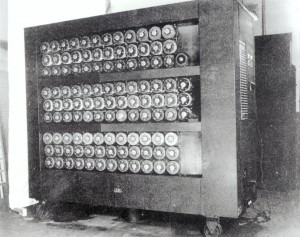
\includegraphics[scale=0.6]{turingbomb}
\caption{Ena od Turingovih bomb}
\label{fig:bomba}
\end{figure}
\end{minipage}
\hfill
\begin{minipage}[b]{0.45\linewidth}
\begin{figure}
\centering
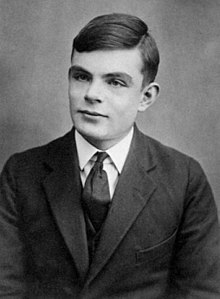
\includegraphics[scale=0.5]{AlanTuring16}
\label{fig:turing}
\caption{Alan Turing, 16 let}
\end{figure}
\end{minipage}
\end{frame}

\begin{frame}{Motivacija}
\end{frame}

\begin{frame}{Ideja je rojena}
\end{frame}

\begin{frame}{Matematične osnove}
\framesubtitle{Modularna aritmetika in kolobar $\Zn$}
\end{frame}

\begin{frame}{Matematične osnove}
\framesubtitle{Funkcija $\varphi$ in Eulerjev izrek}
\end{frame}

\begin{frame}{Matematične osnove}
\framesubtitle{Polinomi in številski sistemi}
\end{frame}

\begin{frame}{Kako deluje?}
\end{frame}

\begin{frame}{Zakaj deluje?}
\end{frame}

\begin{frame}{Načrt napada}
\end{frame}

\begin{frame}{Napad 1:}
\framesubtitle{Faktorizacija $n$, če poznamo $\phi(n)$}
\end{frame}

\begin{frame}{Napad 2:}
\framesubtitle{Kaj če sta $p$ in $q$ blizu skupaj?}
\end{frame}

\begin{frame}{Napad 3:}
\framesubtitle{Faktorizacija $n$, če poznamo $d$, oz. napad na skupen modul}
\end{frame}

\begin{frame}{Napad 4:}
\framesubtitle{Chosen-Ciphertext Attack}
\end{frame}

\begin{frame}{Napad 5:}
 \framesubtitle{Napad na majhen šifrirni eksponent $e$}
\end{frame}

\begin{frame}{Napad 6:}
\framesubtitle{Napad na majhen prostor sporočil}
\end{frame}

\begin{frame}{Napad 7:}
\framesubtitle{Napad na majhen dešifrirni eksponent $d$}
\end{frame}

\begin{frame}{Napad 8:}
\framesubtitle{Cikličen napad}
\end{frame}

\begin{frame}{Uporaba}
\end{frame}

\begin{frame}{Viri}
\end{frame}



\end{document}